\renewcommand\thechapter{\Roman{chapter}}
\chapter{MÉTODO} \label{ch:metodo} \thispagestyle{fancy}
\renewcommand\thechapter{\arabic{chapter}}
%%%%%%%%%%%%%%%%%%%%%%%%%%%%%%%%%%%%%%%%%%%%%%%%%%%%%%%%%%%%%%%%%%%%%%%%%%%%
En este capítulo se abordará la ruta metodológica que se llevó a cabo para realizar el proyecto. Primero, se indicará el sujeto de estudio. Después, se mostrará un diagrama de flujo y la explicación de cada etapa del proyecto. Por último, se enlistan los materiales y herramientas utilizados en el trabajo.


\section{Sujeto}
\begin{itemize}
\item Investigadores e ingenieros del área de desarrollo de hardware. 
\end{itemize}

\section{Procedimiento}

\begin{figure}[!h]
\centering
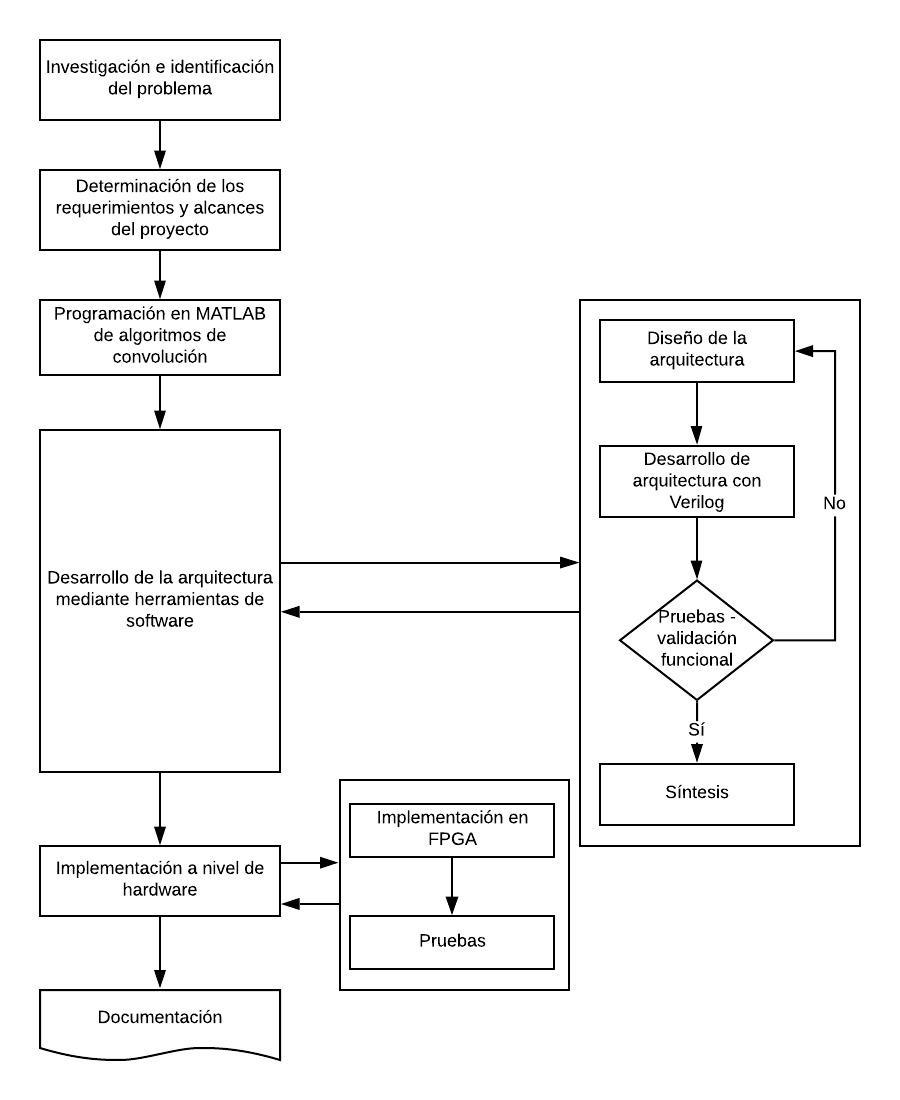
\includegraphics[width=0.8\textwidth, height=0.9\textheight]{./figs/procedimiento}\\
\caption{Diagrama de flujo}
\label{diagramaflujo}
\end{figure}

\newpage
En la figura \ref{diagramaflujo} se muestra la ruta metodológica a seguir para desarrollar el co-procesador para la convolución. A continuación se describre cada uno de los pasos. 

\subsection{Identificación del problema e investigación}
Se determina la problemática, en base al análisis del entorno actual de la computación, al cual se le buscará solución con el proyecto que se presenta en este trabajo. El problema que se aborda es la necesidad de encontrar alternativas a las tendencias actuales para el procesamiento de señales con mejores prestaciones de cómputo intensivo y con menor consumo de potencia, específicamente para la operación de la convolución.

Además, se recopila información acerca de procesadores para la convolución en bases de datos de artículos científicos y en libros técnicos. Esta información de trabajos similares al desarrollado en este documento servirá para comparar el rendimiento de la arquitectura propuesta en este trabajo, además se analiza qué se puede mejorar con respecto a estos trabajos existentnes en la actualidad. Esta etapa consiste en la investigación del estado del arte, es decir, cuál es la situación actual de esta tecnología.

\subsection{Determinación de los requerimientos y alcances del proyecto}
Se determina cuáles son los alcances y delimitaciones del proyecto, es decir hasta dónde se va a investigar y desarrollar. El diseño del procesador se limitará a diseñar  la arquitectura para un coprocesador para la convolución. Se implementará en un FPGA y se verificará a través de un entorno de simulación con la ayuda de MATLAB. En este proyecto las limitaciones son el tiempo disponible, dinero, recursos y licencias.

\subsection{Programación en MATLAB de algoritmos de convolución}
Se desarrollan diferentes algoritmos existentes para resolver la operación de la convolución utilizando el lenguaje de programación MATLAB. La finalidad de esta etapa es comparar el rendimiento en tiempo de ejecución y uso de recursos de memoria de los diferentes algoritmos y analizar las ventajas y desventajas de cada uno de ellos. 

\subsection{Desarrollo de la arquitectura mediante herramientas de software}
Se desarrolla la arquitectura utilizando metodologías de diseño y herramientas de software que facilitan el desarrollo de hardware. 

\subsubsection{Diseño de la arquitectura}
Mediante el uso de la metodología Top-Down y en base a las arquitecturas de la actualidad se desarrolla una arquitectura capaz de realizar la operación de la convolución con un menor consumo de potencia y con una velocidad de procesamiento comparable con las arquitecturas modernas.  

\subsubsection{Desarrollo de arquitectura con Verilog}
Con la ayuda de un lenguaje de descripción de hardware, en este caso Verilog, se describe la arquitectura digital en Xilinx ISE 14.7. Se describen los diferentes bloques que forman parte de la arquitectura, posteriormente se unen estos elementos con un top level. 

\subsubsection{Pruebas - validación funcional}
Se simula la arquitectura mediante el uso de test bench. Los resultados se comparan con resultados obtenidos con la función predeterminada de MATLAB llamada conv() la cual realiza la operación de la convolución de dos señales.

\subsubsection{Síntesis}
Se realiza la síntesis lógica del código. Este paso consiste en convertir la descripción de hardware especificada mediante Verilog en una implementación de diseño en término de compuertas lógicas, generando un archivo de flujo de bits (.bit) que sirve para programar el FPGA. 

\subsection{Implementación a nivel de hardware}
En esta etapa se programa el FPGA y se realizan pruebas para comprobar la correcta operación de la arquitectura propuesta. 

\subsubsection{Implementación en FPGA}
Una vez que se cuenta con la arquitectura sintetizada, se programa el archivo de flujo de bits en el FPGA utilizando el software Digilent Adept. Esto sirve para configurar el FPGA para que lleve a cabo la operación de la convolución.

\subsubsection{Pruebas}
Se realizan pruebas al hardware mediante una interfaz de comunicación serial la cual conecta al FPGA con una PC. Se alimenta al FPGA con dos señales, las cuales se convolucionan en la arquitectura digital, y el FPGA da como resultado una tercera señal. Este resultado se compara con resultados obtenidos bajo un ambiente conocido en MATLAB y sirve para comprobar que el sistema digital está funcionando de manera correcta. Se realizan pruebas de velocidad de procesamiento y consumo de potencia.

\subsection{Documentación}
Se realiza un trabajo escrito en el cual se documentan los aspectos más relevantes del proyecto. Primero, se da una introducción al proyecto y se pone en contexto al lector, después se presenta el trabajo realizado así como se describe a detalle la forma en que se realizó cada etapa, por último, se presentan los resultados obtenidos así como un análisis de los mismos. 

\section{Materiales y Herramientas}
\begin{itemize}
\item Laptop Dell Inspiron 13-5378
\item MathWorks MATLAB R2015a
\item Xilinx ISE 14.7
\item Digilent Adept
\color{red}
\item agregar los que faltan (FPGA, OS(?))
\end{itemize}
